\documentclass[11pt]{article}
\usepackage[utf8x]{inputenc}
\usepackage[english]{babel}
\usepackage{graphicx}
\usepackage{wrapfig}
\usepackage[margin=2cm, tmargin=2cm]{geometry}
\usepackage{color}
\usepackage{hyperref}
\usepackage{paralist}
\usepackage{wrapfig}
\usepackage{multicol}
\usepackage[normalem]{ulem}

\begin{document}
\noindent Prénom: \hfill {\scshape cyber} 2, {\scshape ensibs} Vannes, 2015-09-21 \\
Nom:
\begin{center}
	{\LARGE{Examen de Réseau}} \\ \vspace{10pt}
	Une page A4 recto/verso de \textbf{notes masnuscrites} est autorisée mais aucune forme de communication ne sera tolérée!
	Les réponses \textbf{courtes} et correctes sont les meilleures. \underline{Pas la peine de philosopher ou débattre} (Français ou Anglais au choix). La notation est à titre informatif et pourrait changer. \\
	Bonne chance!
\end{center}

\section{Design de sous-réseaux (10 pts)}
	Dans cet exercice vous devez designez plusieurs sous-réseaux. En commençant à 172.17.0.0, donner pour chacun des sous réseaux (aucun schéma attendu, mais cela pourrait vous aider):
	\begin{itemize}
		\item Le masque de sous-réseaux et nombre maximum d'hôtes,
		\item L'adresse IP du réseau,
		\item La première adresse IP d'hôte du réseau,
		\item La dernière adresse IP d'hôte du réseau,
		\item L'adresse IP de broadcast.
		%\item the CIDR of the "super-network".
	\end{itemize}
	Les sous-réseaux a designé sont:
	\begin{enumerate}
		\item 1000 machines pour les étudiants,
		\item 30 machines pour les services réseaux (serveur DNS, web, NAS...),
		\item 40 machines pour le laboratoire réseau,
		\item 500 machines pour enseignants et personnels,
		\item 14 machines à des fins d'expérimentation.
	\end{enumerate}
Utilisez le tableau \ref{tab:design} de la page 4.

\section{Modèle OSI (2 pts)}
	Donnez le nom et un rapide aperçu des 4 premières couches réseaux.
\pagebreak

\section{Routage (2 pts)}
	\subsection{Définitions}
		Quelle est la définition des termes: \emph{routeur}, \emph{algorithme de routage} et \emph{transmission (de packets)}? (Il est autorisé de réunir les trois définitions en une seule phrase).
\vspace{3cm}

	\subsection{NIC suivante?}
		\begin{table}[h]
		  \centering
		      \begin{tabular}{llll}
		      		\verb+Route #+	&	\verb+Destination+	& \verb+Genmask+		& \verb+Iface+ \\
		      		R0				&	\verb+0.0.0.0+ 		& \verb+/0+		 		& \verb+s0+ \\
		      		R1				&	\verb+10.0.0.0+		& \verb+/8+				& \verb+eth0+ \\
		      		R2				&	\verb+212.27.60.0+	& \verb+/22+			& \verb+s1+ \\
		      		R3				&	\verb+80.10.200.0+	& \verb+/22+			& \verb+s2+ \\
		      		R4				&	\verb+192.168.0.0+	& \verb+255.255.255.0+	& \verb+eth1+ \\
		      		R5				&	\verb+192.168.3.0+	& \verb+255.255.255.0+	& \verb+eth0+ \\
		      		R6				&	\verb+192.168.5.0+	& \verb+255.255.255.128+& \verb+eth1+ \\
		      \end{tabular}
		      \caption{Routing table}
		  \label{tab:routing}
		\end{table}

		D'après la table de routage \ref{tab:routing}:
		\begin{itemize}
			\item Quel est le détail manquant ?
			\item Où seront transmis les packets ayant comme destination:
			\begin{itemize}
				\item 198.41.191.47?
				\item 192.168.4.3?
				\item 192.168.1.1?
				\item 80.10.201.0?
				\item 80.10.210.0?
				\item 10.128.0.4?
				\item 212.27.61.1?
			\end{itemize}
			\item Est-il possible d'aggréger des routes? Si oui, lesquelles?
		\end{itemize}

\pagebreak
\section{Quelle couche est-ce ? (2 pts)}
	Comlétez le tableau \ref{tab:protocol}, en incluant entre parenthèses le port par défaut s'il existe) avec : \sout{HTTP}, HTTPS, TCP, UDP, MAC, IP, telnet, ssh, ftp, IEEE 802.11, IEEE 802.15.2, DNS, SIP, TLS, ICMP, IS-IS, RIP.
	\subsection{Next NIC?}
		\renewcommand{\arraystretch}{1.5}
			\begin{table}[h]
			%  \centering
			      \begin{tabular}{l|l}
			      		\verb+Layer+	&	\verb+Protocols+	\\ \hline
						\verb+*+		&	\\
			      		7				&	HTTP(80),			\\
			      		6				&	\\
			      		5				&	\\
			      		4				&	\\
			      		3				&	\\
			      		2				&	\\
			      		1				&	\\
			      \end{tabular}
			      \caption{Protocol table}
			  \label{tab:protocol}
			\end{table}
		\renewcommand{\arraystretch}{1.0}

	\section{Qui est-ce? (2 pts)}
		Que pouvez-vous déduire des deux packets capturés présents sur la figure \ref{fig:dns}?
		\begin{figure}[h]
			\begin{center}
				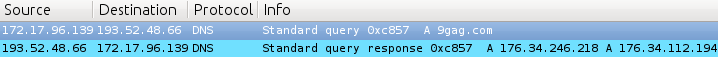
\includegraphics[width=18cm]{dns.png}
				\caption{Two lonely packets}
				\label{fig:dns}
			\end{center}
		\end{figure}
		\vspace{1cm}

\section{Question bonus (0.5 pts)}
	\subsection{DEF CON 22 Hacking Conference}
		Qu'avez-vous appris en regardant la vidéo nommée \emph{Blinding The Surveillance State By Christopher Soghoian}?
\pagebreak

You may want not to write the whole IP addresses but only the changing bytes.
\renewcommand{\arraystretch}{1.5}
\setlength{\tabcolsep}{14pt}
	\begin{table}[h]
	  \centering
		  \begin{tabular}{|l|l|l|l|l|l|l|}
			  \hline
				Network ID	&	Mask (CIDR)	& \# hosts	& Network	&	First node	&	Last node	&	Broadcast	\\ \hline
				&&&&&&	\\ \hline
				&&&&&&	\\ \hline
				&&&&&&	\\ \hline
				&&&&&&	\\ \hline
				&&&&&&	\\ \hline
				&&&&&&	\\ \hline
				&&&&&&	\\ \hline
				&&&&&&	\\ \hline
				&&&&&&	\\ \hline
				&&&&&&	\\ \hline
				&&&&&&	\\ \hline
		  \end{tabular}
		  \caption{Designed networks}
	  \label{tab:design}
	\end{table}
\renewcommand{\arraystretch}{1.0}
\end{document}
